\documentclass[a4paper]{article}
\usepackage{geometry}
\usepackage{graphicx}
\usepackage{natbib}
\usepackage{amsmath}
\usepackage{amssymb}
\usepackage{amsthm}
\usepackage{paralist}
\usepackage{epstopdf}
\usepackage{tabularx}
\usepackage{longtable}
\usepackage{multirow}
\usepackage{multicol}
\usepackage[hidelinks]{hyperref}
\usepackage{fancyvrb}
\usepackage{algorithm}
\usepackage{algorithmic}
\usepackage{float}
\usepackage{paralist}
\usepackage[svgname]{xcolor}
\usepackage{enumerate}
\usepackage{array}
\usepackage{times}
\usepackage{url}
\usepackage{fancyhdr}
\usepackage{comment}
\usepackage{environ}
\usepackage{times}
\usepackage{textcomp}
\usepackage{caption}
\usepackage{multirow}

\usepackage{pgfplots}
\pgfplotsset{compat=1.16}


\urlstyle{rm}

\setlength\parindent{0pt} % Removes all indentation from paragraphs
\theoremstyle{definition}
\newtheorem{definition}{Definition}[]
\newtheorem{conjecture}{Conjecture}[]
\newtheorem{example}{Example}[]
\newtheorem{theorem}{Theorem}[]
\newtheorem{lemma}{Lemma}
\newtheorem{proposition}{Proposition}
\newtheorem{corollary}{Corollary}


\floatname{algorithm}{Procedure}
\renewcommand{\algorithmicrequire}{\textbf{Input:}}
\renewcommand{\algorithmicensure}{\textbf{Output:}}
\newcommand{\abs}[1]{\lvert#1\rvert}
\newcommand{\norm}[1]{\lVert#1\rVert}
\newcommand{\RR}{\mathbb{R}}
\newcommand{\CC}{\mathbb{C}}
\newcommand{\Nat}{\mathbb{N}}
\newcommand{\br}[1]{\{#1\}}
\DeclareMathOperator*{\argmin}{arg\,min}
\DeclareMathOperator*{\argmax}{arg\,max}
\renewcommand{\qedsymbol}{$\blacksquare$}

\definecolor{dkgreen}{rgb}{0,0.6,0}
\definecolor{gray}{rgb}{0.5,0.5,0.5}
\definecolor{mauve}{rgb}{0.58,0,0.82}

\newcommand{\Var}{\mathrm{Var}}
\newcommand{\Cov}{\mathrm{Cov}}

\newcommand{\vc}[1]{\boldsymbol{#1}}
\newcommand{\xv}{\vc{x}}
\newcommand{\Sigmav}{\vc{\Sigma}}
\newcommand{\alphav}{\vc{\alpha}}
\newcommand{\muv}{\vc{\mu}}

\newcommand{\red}[1]{\textcolor{red}{#1}}
\renewcommand\vec[1]{\mathbf{#1}}

\def\x{\mathbf x}
\def\y{\mathbf y}
\def\w{\mathbf w}
\def\v{\mathbf v}
\def\E{\mathbb E}
\def\V{\mathbb V}

% TO SHOW SOLUTIONS, include following (else comment out):
\newenvironment{soln}{
    \leavevmode\color{blue}\ignorespaces
}{}


\hypersetup{
%    colorlinks,
    linkcolor={red!50!black},
    citecolor={blue!50!black},
    urlcolor={blue!80!black}
}

\geometry{
  top=1in,            % <-- you want to adjust this
  inner=1in,
  outer=1in,
  bottom=1in,
  headheight=3em,       % <-- and this
  headsep=2em,          % <-- and this
  footskip=3em,
}


\pagestyle{fancyplain}
\lhead{\fancyplain{}{Homework 3}}
\rhead{\fancyplain{}{CS 760 Machine Learning}}
\cfoot{\thepage}

\title{\textsc{Homework 3}} % Title

%%% NOTE:  Replace 'NAME HERE' etc., and delete any "\red{}" wrappers (so it won't show up as red)

\author{
\red{NAME} \\
\red{\#}\\
} 


\begin{filecontents}{roc1.dat}
  x      f(x)
  0       0
  0 0.16
  0 0.33  
  0 0.5
  0.25  0.5
  0.25  0.66
  0.5 0.66
  0.5 0.83
  0.75  0.83
  0.75  1
  1 1
\end{filecontents}


\date{}

\begin{document}

\maketitle


\textbf{Instructions:}
Use this latex file as a template to develop your homework.
Submit your homework on time as a single zip (containing the pdf and the code) file to Canvas. Please, check Piazza for updates about the homework. It is recommended that you use Python for your solutions. You are allowed to use the libraries {\tt numpy}, {\tt matplotlib} and {\tt pandas}.
\section{Questions (60 pts)}
\begin{enumerate}
  \item (9 pts) Explain whether each scenario is a classification or regression problem. Additionally, provide the number of data points ($n$) and the number of features ($p$).

        \begin{enumerate}
          \item (3 pts) We collect a set of data on the top 500 firms in the US. For each firm, we record profit, number of employees, industry and the CEO salary. We are interested in predicting CEO salary with given factors.

                \begin{soln}  Regression problem where the output is a continuous/numeric value (CEO Salary); Where f = 3 (out prediction inference affected by the following features: profit, number of employees, and industry); n = 500 (500 firms provide out labeled data);  \end{soln}

          \item (3 pts) We are considering launching a new product and wish to know whether it will be a success or a failure. We collect data on 20 similar products that were previously launched. For each product, we have recorded whether it was a success or failure, price charged for the product, marketing budget, competition price, and ten other variables.

                \begin{soln}  Classification problem as the predicted output is a nominal value (success/failure can be represented as binary positive/negative output). f = 13 (as 3 named + 10 other input values are provided). n = 20 (colleced labeled data that will be examined is of 20 similar products).  \end{soln}

          \item (3 pts) We are interested in predicting the \% change in the US dollar in relation to the weekly changes in the world stock markets. Hence, we collect weekly data for all of 2012. For each week, we record the \% change in the dollar, the \% change in the US market, the \% change in the British market, and the \% change in the German market.

                \begin{soln}  Regression problem as we are predicting \% change in US dollar, which is a numeric quantitative value (percentage change of 0 through 100 that can also possibly be a fraction percentage); f = 3 (each recorded instance includes values of \% change for each of 3 interested markets); n = 52 (assuming data is collected for complete weeks of the year 2012, then we will end up with 52 weeks each representing a data point). \end{soln}


        \end{enumerate}

  \item (6 pts) The table below provides a training dataset containing six observations, three predictors, and one qualitative response variable.

        \begin{center}
          \begin{tabular}{ c  c  c  c}
            \hline
            $X_{1}$ & $X_{2}$ & $X_{3}$ & $Y$   \\ \hline
            0       & 3       & 0       & Red   \\
            -2      & 0       & 0       & Red   \\
            0       & -1      & 3       & Red   \\
            0       & 1       & 2       & Green \\
            -1      & 0       & 1       & Green \\
            1       & -1      & 1       & Red   \\
            \hline
          \end{tabular}
        \end{center}

        Suppose we wish to use this dataset to make a prediction for $Y$ when $X_{1} = X_{2} = X_{3} = 0$ using $K$-nearest neighbors.

        \begin{enumerate}
          \item (2 pts) Compute the Euclidean distance between each observation and the test point, $X_{1} = X_{2} = X_{3}=0$.
                \begin{soln}
                  \begin{align}
                    x^{test\ point} & = \langle {0, 0, 0} \rangle                           \\
                    \vert x^1 \vert & = \sqrt[]{(3-0)^2} = 3                                \\
                    \vert x^2 \vert & = \sqrt[]{(-2-0)^2 } = 2                              \\
                    \vert x^3 \vert & = \sqrt[]{(-1-0)^2 + (3-0)^2 } = \sqrt[]{10}          \\
                    \vert x^4 \vert & = \sqrt[]{(1-0)^2 + (2-0)^2 } = \sqrt[]{5}            \\
                    \vert x^5 \vert & = \sqrt[]{(-1-0)^2 +  (1)^2 } = \sqrt[]{2}            \\
                    \vert x^6 \vert & = \sqrt[]{(1-0)^2 + (-1-0)^2 + (1-0)^2 } = \sqrt[]{3}
                  \end{align}
                \end{soln}
          \item (2 pts) What is our prediction with $K=1$? Why?

                \begin{soln}
                  The order by distance of instances to the test point is: $x^5$,$x^6$,$x^4$, $x^3$, $x^2$, $x^1$; Thus, $x^5$ is the closest neighbor to the test point.Its given label is `Green', therefore the 1NN algorithm will predict the test point to be `Green`.
                \end{soln}

          \item (2 pts) What is our prediction with $K=3$? Why?

                \begin{soln}
                  3-NN algorithm will choose $x^5$, $x^6$, $x^4$ as closest neighbors. Those have values of {G, R, G}  respectively. Assuming the majority label is to be picked, then {2 Green $>$ 1 Red} $=>$ test point predicted as majority class `Green`.
                \end{soln}

        \end{enumerate}

  \item (12 pts) When the number of features $p$ is large, there tends to be a deterioration in the performance of kNN and other local approaches that perform prediction using only observations that are near the test observation for which a prediction must be made. This phenomenon is known as the curse of dimensionality, and it ties into the fact that non-parametric approaches often perform poorly when $p$ is large.

        \begin{enumerate}
          \item (2 pts) Suppose that we have a set of observations, each with measurements on $p =1$ feature, $X$. We assume that $X$ is uniformly (evenly) distributed on $[0, 1]$. Associated with each observation is a response value. Suppose that we wish to predict the response of a test observation using only observations that are within 10\% of the range of $X$ closest to that test observation. For instance, in order to predict the response for a test observation with $X =0.6$, we will use observations in the range $[0.55, 0.65]$. On average, what fraction of the available observations will we use to make the prediction?

                \begin{soln}
                  At least for observations with defined 10\% range around it, then we will use 10\% of observation equivalent to 0.1 length. Specificaly, $x \in [0.05, 0.95]$ the interval would be $[x-0.05, x+0.05]$, with a length of 0.1 combined from left and right portion, equivalent to fraction of 10\%.  \\
                  While for the edge observations the range will be less than 0.1 length. For $x<0.05$ the the interval will be $[0, 0.05]$, which is a fraction of $x+0.05$. And for $x \in [0.95, 1]$ the fraction would be $0.05+(1-x) = 1.05 - x$ . Thus, the piecewise function represent the fraction of observations used for to make a predition for each observation point.

                  \[
                    fraction(x) = \left\{
                    \begin{array}{@{}l@{\thinspace}l}
                      $x + 0.05$ & : \text{} \text{} $[0, 0.05]$    \\
                      $0.1$      & : \text{}  \text{}$[0.05, 0.95]$ \\
                      $1.05 - x$ & : \text{}  \text{}$[0.95, 1]$    \\
                    \end{array}
                    \right.
                  \]

                  By finding the mean of f(x) value using using mean value theorem for integrals (integration of the individual ranges and dividing by range $1-0$) we can get the average fraction of observations used for prediction: $average fraction = 0.0975$

                \end{soln}



          \item (2 pts) Now suppose that we have a set of observations, each with measurements on $p =2$ features, $X1$ and $X2$.
                We assume that $(X1,X2)$ are uniformly (evenly) distributed on $[0, 1] \times [0, 1]$.  Associated with each observation is a response value.
                Suppose that we wish to predict the response of a test observation using only observations that are within 10\% of the range of $X1$ and within 10\% of the range of $X2$ closest to that test observation. For instance, in order to predict the response for a test observation with $X1 =0.6$ and $X2 =0.35$, we will use observations in the range $[0.55, 0.65]$ for $X1$ and in the range $[0.3, 0.4]$ for $X2$. On average, what fraction of the available observations will we use to make the prediction?

                \begin{soln}
                  Building on the previous answer, for each feature $X_1$ \& $X_2$ the fraction of average observations used is 0.0975 out of $[0,1]$ range. The combined fractions would represent the average of observations used to make a prediction. $Average fraction = 0.0975 \cdot 0.0975 = 0.0095 $
                \end{soln}

          \item (2 pts) Now suppose that we have a set of observations on $p = 100$ features. Again, the observations are uniformly distributed on each feature, and again each feature ranges in value from 0 to 1. We wish to predict the response of a test observation using observations within the 10\% of each feature’s range that is closest to that test observation. What fraction of the available observations will we use to make the prediction?

                \begin{soln}  We will repeat the same process for $p=2$ but with $p=100$. \\ $Average fraction = 0.0975^{100} = \text{impractical minut fraction} = 0$ \end{soln}

          \item (3 pts) Using your answers to parts (a)–(c), argue that a drawback of kNN when $p$ is large is that there are very few training observations “near” any given test observation.

                \begin{soln}
                  From our observation for 1 feature we could use $0.0975 = 9.75\%$ of trainng observatoins on average for predicting a test observation. While for point in 2 dimensions $0.95\%$ of training data around it can be used. As feature dimensions increase we exponentially decay the number of observations considered on importance around the test point. The general rule would be $$\lim_{p\to\infty}(0.0975)^p = 0$$ Even more so, can be generalized to any fraction.
                  \\Therefore the k-NN using labeled data with large number of features will not be accurate, as the supposed k-nearest points for a given test are likely to be far away and meaningless.

                \end{soln}

          \item (3 pts) Now suppose that we wish to make a prediction for a test observation by creating a $p$-dimensional hypercube centered around the test observation that contains, on average, 10\% of the training observations. For $p =1, 2$, and $100$, what is the length of each side of the hypercube? Comment on your answer.

                \begin{soln} Each p is an additional dimension for the hypercube. If for 1-dimension we map 0.1 of the entire 1 length, and for 2-dimension we map the area as a fraction of $[0,1]\cdot[0,1]$ area. Then in p-dimension $[0,1]^p$ we will consider the fraction of a volume to represent the training observations used for prediction, i.e. 10\% training observations would be equivalent to 10\% of volume.
                  $$V = (\text{side length})^p$$ then:
                  $$\text{side length} = V^{1/p}$$
                  \\
                  Thus,\\
                  p = 1:  $\text{side length} = 0.1^{1/1} = 0.1 $\\
                  p = 2:  $\text{side length} = 0.1^{1/2} \approxeq 0.31$\\
                  p = 100:  $\text{side length} = 0.1^{1/100} \approxeq 0.97$
                \end{soln}

        \end{enumerate}

  \item (6 pts) Suppose you trained a classifier for a spam detection system. The prediction result on the test set is summarized in the following table.
        \begin{center}
          \begin{tabular}{l l | l l}
                                          &          & \multicolumn{2}{l}{Predicted class}            \\
                                          &          & Spam                                & not Spam \\
            \hline
            \multirow{2}{*}{Actual class} & Spam     & 8                                   & 2        \\
                                          & not Spam & 16                                  & 974
          \end{tabular}
        \end{center}

        Calculate
        \begin{enumerate}
          \item (2 pts) Accuracy
                \begin{soln}  $$\text{Accuracy} = \dfrac{TP + TN}{TP + FN + FP + TN} = \dfrac{8 + 974}{8+2+16+074} = 0.982 $$ \end{soln}
          \item (2 pts) Precision
                \begin{soln}  $$\text{Precision} = \dfrac{TP}{TP+FP} = \dfrac{8}{8+16} = 1/3 $$. \end{soln}
          \item (2 pts) Recall
                \begin{soln}   $$\text{Recall} = \dfrac{TP}{TP+FN} = \dfrac{8}{8+2} = 0.8 $$ \end{soln}
        \end{enumerate}


  \item (9 pts) Again, suppose that you trained a classifier for a spam filter. The prediction result on the test set is summarized in the following table. Here, {\tt +} represents {\tt spam}, and {\tt -} means {\tt not spam}.

        \begin{center}
          \begin{tabular}{ c  c }
            \hline
            Confidence positive & Correct class \\ \hline
            0.95                & +             \\
            0.85                & +             \\
            0.8                 & +             \\
            0.7                 & -             \\
            0.55                & +             \\
            0.45                & -             \\
            0.4                 & +             \\
            0.3                 & -             \\
            0.2                 & +             \\
            0.1                 & -             \\
            \hline
          \end{tabular}
        \end{center}

        \begin{enumerate}
          \item (6pts) Draw an ROC curve based on the above table.

                \begin{soln}
                  Let t := confidence threshold. If confidence positive value $\ge t$, then the model would classify the observation as spam (+). Thus for each splitting threshold $t$ in confidence positive we get the following confusion matrices, FP(t), and TP(t) rates:

                  \begin{center}
                    \captionof{table}{$t = 0.1$} \label{tab:title}
                    \begin{tabular}{l l | l l}
                                                    &          & \multicolumn{2}{l}{Predicted class}            \\
                                                    &          & Spam                                & not Spam \\
                      \hline
                      \multirow{2}{*}{Actual class} & Spam     & 6                                   & 0        \\
                                                    & not Spam & 4                                   & 0
                    \end{tabular}
                  \end{center}
                  $TP(t) =  1$\\
                  $FP(t) = 1$

                  \begin{center}
                    \captionof{table}{$t = 0.2$} \label{tab:title}
                    \begin{tabular}{l l | l l}
                                                    &          & \multicolumn{2}{l}{Predicted class}            \\
                                                    &          & Spam                                & not Spam \\
                      \hline
                      \multirow{2}{*}{Actual class} & Spam     & 6                                   & 0        \\
                                                    & not Spam & 3                                   & 1
                    \end{tabular}
                  \end{center}
                  $TP(t) = 1$\\
                  $FP(t) = 0.75$

                  \begin{center}
                    \captionof{table}{$t = 0.3$} \label{tab:title}
                    \begin{tabular}{l l | l l}
                                                    &          & \multicolumn{2}{l}{Predicted class}            \\
                                                    &          & Spam                                & not Spam \\
                      \hline
                      \multirow{2}{*}{Actual class} & Spam     & 5                                   & 1        \\
                                                    & not Spam & 3                                   & 1
                    \end{tabular}
                  \end{center}
                  $TP(t) = 0.83 $\\
                  $FP(t) = 0.75$

                  \begin{center}
                    \captionof{table}{$t = 0.4$} \label{tab:title}
                    \begin{tabular}{l l | l l}
                                                    &          & \multicolumn{2}{l}{Predicted class}            \\
                                                    &          & Spam                                & not Spam \\
                      \hline
                      \multirow{2}{*}{Actual class} & Spam     & 5                                   & 1        \\
                                                    & not Spam & 2                                   & 2
                    \end{tabular}
                  \end{center}
                  $TP(t) = 0.83$\\
                  $FP(t) = 0.5$

                  \begin{center}
                    \captionof{table}{$t = 0.45$} \label{tab:title}
                    \begin{tabular}{l l | l l}
                                                    &          & \multicolumn{2}{l}{Predicted class}            \\
                                                    &          & Spam                                & not Spam \\
                      \hline
                      \multirow{2}{*}{Actual class} & Spam     & 4                                   & 2        \\
                                                    & not Spam & 2                                   & 2
                    \end{tabular}
                  \end{center}
                  $TP(t) = 0.66$\\
                  $FP(t) = 0.5$

                  \begin{center}
                    \captionof{table}{$t = 0.55$} \label{tab:title}
                    \begin{tabular}{l l | l l}
                                                    &          & \multicolumn{2}{l}{Predicted class}            \\
                                                    &          & Spam                                & not Spam \\
                      \hline
                      \multirow{2}{*}{Actual class} & Spam     & 4                                   & 2        \\
                                                    & not Spam & 1                                   & 3
                    \end{tabular}
                  \end{center}
                  $TP(t) = 0.66$\\
                  $FP(t) = 0.25$

                  \begin{center}
                    \captionof{table}{$t = 0.7$} \label{tab:title}
                    \begin{tabular}{l l | l l}
                                                    &          & \multicolumn{2}{l}{Predicted class}            \\
                                                    &          & Spam                                & not Spam \\
                      \hline
                      \multirow{2}{*}{Actual class} & Spam     & 3                                   & 3        \\
                                                    & not Spam & 1                                   & 3
                    \end{tabular}
                  \end{center}
                  $TP(t) = 0.5$\\
                  $FP(t) = 0.25$

                  \begin{center}
                    \captionof{table}{$t = 0.8$} \label{tab:title}
                    \begin{tabular}{l l | l l}
                                                    &          & \multicolumn{2}{l}{Predicted class}            \\
                                                    &          & Spam                                & not Spam \\
                      \hline
                      \multirow{2}{*}{Actual class} & Spam     & 3                                   & 3        \\
                                                    & not Spam & 0                                   & 4
                    \end{tabular}
                  \end{center}
                  $TP(t) = 0.5$\\
                  $FP(t) = 0$

                  \begin{center}
                    \captionof{table}{$t = 0.85$} \label{tab:title}
                    \begin{tabular}{l l | l l}
                                                    &          & \multicolumn{2}{l}{Predicted class}            \\
                                                    &          & Spam                                & not Spam \\
                      \hline
                      \multirow{2}{*}{Actual class} & Spam     & 2                                   & 4        \\
                                                    & not Spam & 0                                   & 4
                    \end{tabular}
                  \end{center}
                  $TP(t) = 0.33$\\
                  $FP(t) = 0$

                  \begin{center}
                    \captionof{table}{$t = 0.95$} \label{tab:title}
                    \begin{tabular}{l l | l l}
                                                    &          & \multicolumn{2}{l}{Predicted class}            \\
                                                    &          & Spam                                & not Spam \\
                      \hline
                      \multirow{2}{*}{Actual class} & Spam     & 1                                   & 5        \\
                                                    & not Spam & 0                                   & 4
                    \end{tabular}
                  \end{center}
                  $TP(t) = 0.16$\\
                  $FP(t) = 0$

                  \begin{center}
                    \captionof{table}{$t = 1.0$} \label{tab:title}
                    \begin{tabular}{l l | l l}
                                                    &          & \multicolumn{2}{l}{Predicted class}            \\
                                                    &          & Spam                                & not Spam \\
                      \hline
                      \multirow{2}{*}{Actual class} & Spam     & 0                                   & 6        \\
                                                    & not Spam & 0                                   & 4
                    \end{tabular}
                  \end{center}
                  $TP(t) = 0$\\
                  $FP(t) = 0$


                  \begin{tikzpicture}
                    \begin{axis}[
                        title={ROC curve},
                        xlabel={$FP(t)$},
                        ylabel={$TP(t)$},
                      ]
                      \addplot [blue,mark=diamond*] table {roc1.dat};
                    \end{axis}
                  \end{tikzpicture}



                \end{soln}

          \item (3pts) (Real-world open question) Suppose you want to choose a tlarhreshold parameter so that mails with confidence positives above the threshold can be classified as spam. Which value will you choose? Justify your answer based on the ROC curve.

                \begin{soln}  The best threshold to choose depends on each use case's relative cost FN \& FP misclassification. For the case of email spam, FN refers to the spam emails that are classified as legit, while FP refers to the legit emails that are classified as spam. From experience, it is more important to prevent legit emails from going to spam (no tolerance to finding important email in the spam folder) than it is to increase the spam hit rate. Therefore, a good tradeoff for accuracy of our model would be $threshold = 0.8$ corresponding to the left corner point. \end{soln}
        \end{enumerate}

  \item (8 pts) In this problem, we will walk through a single step of the gradient descent algorithm for logistic regression. Assume two-dimensional input.
        Recap:
        $$f(\vec x;\vec v, b) = \sigma(\vec v \cdot \vec x + b) \;,$$
        where $\sigma$ is the logistic function discussed in class.
        $$\text{Cross-entropy loss: } L(\hat{y}, y) = -[y \log  \hat{y} + (1-y)\log(1-\hat{y})]$$
        $$\text{The single update step: } \vec w^{(t+1)} = \vec w^{(t)} - \eta \nabla_{\vec w} L(f(\vec x;\vec w), y),\text{ where } \vec w=[\vec v_{1}, \vec v_{2}, b]^T $$

        Now given
        $$ \text{Initial parameters : } \vec v_{1}=b=0,\vec v_{2}=1,(\Rightarrow \vec w^{(0)}=[0, 1, 0]))$$
        $$ \text{Learning rate: }\eta=0.1$$
        $$ \text{Data example: } \vec x=[3, 2], y=1$$

        \begin{enumerate}
          \item (4 pts) Compute the first gradient $\nabla_{\vec w} L(f(\vec x;\vec w), y)$.

                \begin{soln}  Solution goes here. \end{soln}

          \item (4 pts) Compute the updated parameter vector $\vec w^{(1)}$ from a single update step.

                \begin{soln}  Solution goes here. \end{soln}
        \end{enumerate}

  \item (10 pts) In this problem, we consider a variant of linear regression with sparse structure. The only difference with standard linear regression is that the hidden regressor vector has at most $k$ non-zero parameters, where the sparsity $k$ is much smaller than the dimension $d$. For example, for $k=2$ and $d=4$, the following parameters are feasible solutions: $\vec w=[0,0,0,0]$, $\vec w=[0,0,0,7]$,
        $\vec w=[0,14,0,21]$, while $\vec w=[1,5,2,7]$ and $\vec w=[1,0,5,8]$ are not.
        \begin{enumerate}
          \item (3 pt) Define the optimization problem for sparse linear regression, i.e., that of finding a sparse vector minimizing the square loss.

                \begin{soln}  Solution goes here. \end{soln}

          \item (7 pts) Can we use (Stochastic) Gradient Descent to minimize this objective? Justify your answer.

                \begin{soln}  Solution goes here. \end{soln}
        \end{enumerate}
\end{enumerate}

\section{Programming (50 pts)}
\begin{enumerate}
  \item (10 pts) Use the entire {\tt D2z.txt} as a training set.  Use Euclidean distance (i.e., $\vec A=\vec I$).
        Visualize the predictions of 1NN on a 2D grid $[-2:0.1:2]\times [-2:0.1:2]$.
        That is, you should produce test points whose first feature goes over $-2, -1.9, -1.8, \ldots, 1.9, 2$, so does the second feature independent of the first feature.
        You should overlay the training set in the plot, just make sure that we can tell which points are training, which are grid.

        The expected figure looks like this.
        \begin{figure}[h]
          \centering
          \includegraphics[width=5cm]{implementation1_expected_result.png}
        \end{figure}


        \begin{figure}[h]
          \centering
          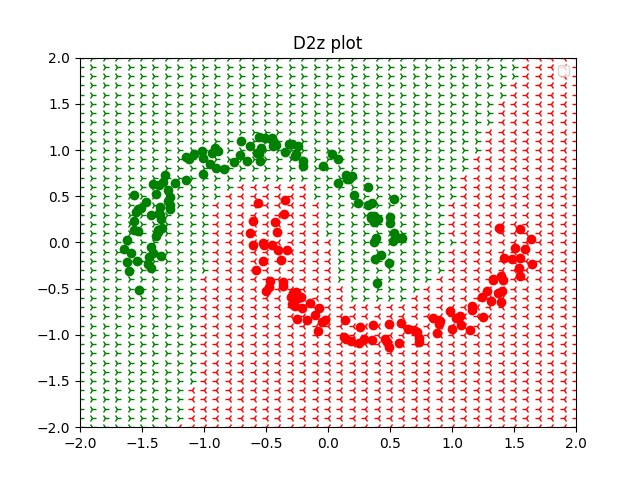
\includegraphics[width=10cm]{1.png}
        \end{figure}


        \paragraph{Spam filter} Now, we will use {\tt emails.csv} as our dataset. The description is as follows.
        \begin{figure}[h]
          \centering
          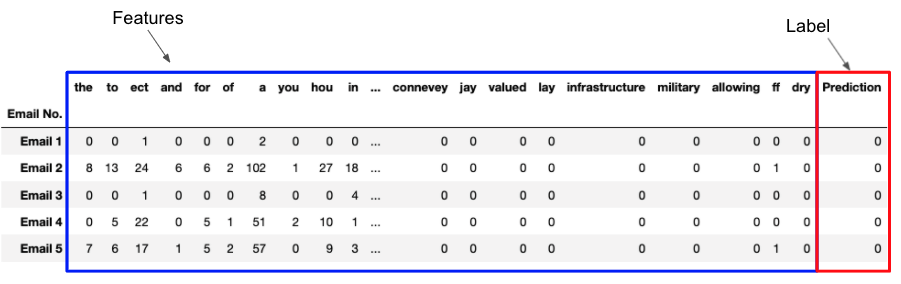
\includegraphics[width=18cm]{email_head.png}
        \end{figure}

        \begin{itemize}
          \item Task: spam detection
          \item The number of rows: 5000
          \item The number of features: 3000 (Word frequency in each email)
          \item The label (y) column name: {\tt Predictor}
          \item For a single training/test set split, use Email 1-4000 as the training set, Email 4001-5000 as the test set.
          \item For 5-fold cross-validation, split dataset in the following way.
                \begin{itemize}
                  \item Fold 1, test set: Email 1-1000, training set: the rest (Email 1001-5000)
                  \item Fold 2, test set: Email 1000-2000, training set: the rest
                  \item Fold 3, test set: Email 2000-3000, training set: the rest
                  \item Fold 4, test set: Email 3000-4000, training set: the rest
                  \item Fold 5, test set: Email 4000-5000, training set: the rest
                \end{itemize}
        \end{itemize}

  \item (10 pts) Implement 1NN and run a 5-fold cross-validation. Report accuracy, precision, and recall in each fold.

        \begin{soln}  Solution goes here. \end{soln}

  \item (10 pts) Implement logistic regression and run a 5-fold cross-validation. Report accuracy, precision, and recall in each fold.

        \begin{soln}  Solution goes here. \end{soln}

  \item (10 pts) Run a 5-fold cross-validation with kNN varying $k$ ($k=1, 3, 5, 7$). Plot the average accuracy versus $k$, and list the average accuracy of each case.
        \begin{soln}  Solution goes here. \end{soln}

  \item (10 pts) Use a single training/test setting. Train kNN ($k=5$) and logistic regression on the training set, and draw ROC curves based on the test set. \\
        Expected figure looks like this.
        \begin{figure}[h!]
          \centering
          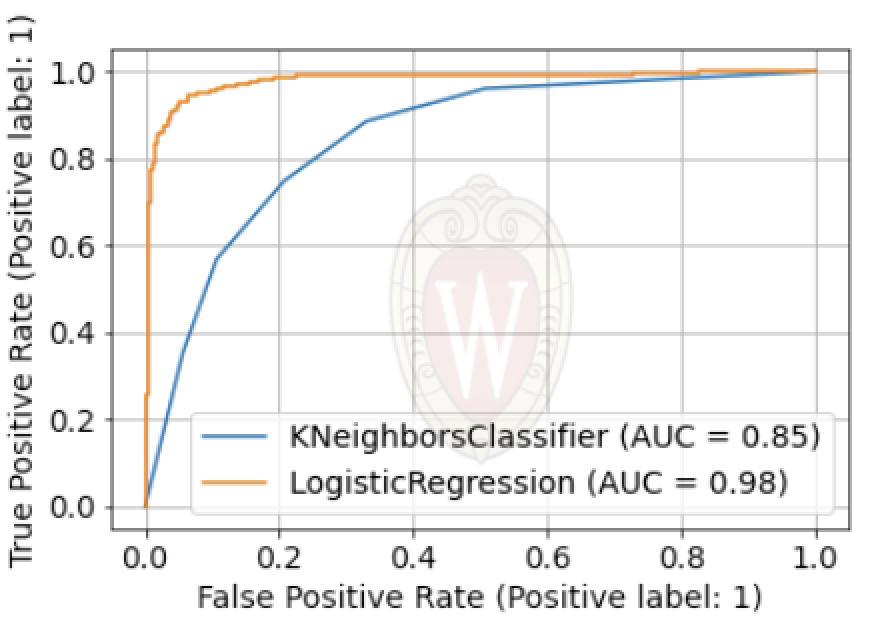
\includegraphics[width=8cm]{roc.png}
        \end{figure}
        Note that the results may differ.

        \begin{soln}  Solution goes here. \end{soln}

\end{enumerate}
\bibliographystyle{apalike}
\end{document}
